%%%%%%%%%%%%%%%%%%%%%%%%%%%%%%%%%%%%%%%%%
% Short Sectioned Assignment
% LaTeX Template
% Version 1.0 (5/5/12)
%
% This template has been downloaded from:
% http://www.LaTeXTemplates.com
%
% Original author:
% Frits Wenneker (http://www.howtotex.com)
%
% License:
% CC BY-NC-SA 3.0 (http://creativecommons.org/licenses/by-nc-sa/3.0/)
%
%%%%%%%%%%%%%%%%%%%%%%%%%%%%%%%%%%%%%%%%%

%----------------------------------------------------------------------------------------
%   PACKAGES AND OTHER DOCUMENT CONFIGURATIONS
%----------------------------------------------------------------------------------------

\documentclass[paper=a4, fontsize=11pt]{scrartcl} % A4 paper and 11pt font size

\usepackage[T1]{fontenc} % Use 10-bit encoding that has 256 glyphs
\usepackage[english]{babel}
\usepackage{polski}
\usepackage[utf8]{inputenc}
\usepackage{amsmath,amsfonts,amsthm} % Math packages
\usepackage{pgfplots} % Math packages
\usepackage{lipsum} % Used for inserting dummy 'Lorem ipsum' text into the template
\usepackage{enumerate}
\usepackage{sectsty} % Allows customizing section commands
\pgfplotsset{compat=1.11}
\allsectionsfont{\centering \normalfont\scshape} % Make all sections centered, the default font and small caps
\usepackage{fancyhdr} % Custom headers and footers
\pagestyle{fancyplain} % Makes all pages in the document conform to the custom headers and footers
\fancyhead{} % No page header - if you want one, create it in the same way as the footers below
\fancyfoot[L]{} % Empty left footer
\fancyfoot[C]{} % Empty center footer
\fancyfoot[R]{\thepage} % Page numbering for right footer
\renewcommand{\headrulewidth}{0pt} % Remove header underlines
\renewcommand{\footrulewidth}{0pt} % Remove footer underlines
\setlength{\headheight}{13.6pt} % Customize the height of the header
\usepackage{listings}

\pgfplotsset{compat=1.10}
\numberwithin{equation}{section} % Number equations within sections (i.e. 1.1, 1.2, 2.1, 2.2 instead of 1, 2, 3, 4)
\numberwithin{figure}{section} % Number figures within sections (i.e. 1.1, 1.2, 2.1, 2.2 instead of 1, 2, 3, 4)
\numberwithin{table}{section} % Number tables within sections (i.e. 1.1, 1.2, 2.1, 2.2 instead of 1, 2, 3, 4)

\setlength\parindent{0pt} % Removes all indentation from paragraphs - comment this line for an assignment with lots of text

%----------------------------------------------------------------------------------------
%   TITLE SECTION
%----------------------------------------------------------------------------------------

\newcommand{\horrule}[1]{\rule{\linewidth}{#1}} % Create horizontal rule command with 1 argument of height

\title{ 
    \normalfont \normalsize 
    \textsc{Politechnika Warszawska} \\ [25pt] % Your university, school and/or department name(s)
    \horrule{0.5pt} \\[0.4cm] % Thin top horizontal rule
    \huge Metody Optymalizacji zadanie 1\\ % The assignment title
    \horrule{2pt} \\[0.5cm] % Thick bottom horizontal rule
}

\author{Mateusz Starzycki} % Your name

\date{\normalsize\today} % Today's date or a custom date

\begin{document}

\maketitle % Print the title

%----------------------------------------------------------------------------------------
%   PROBLEM 1
%----------------------------------------------------------------------------------------

\newpage
\section{Zadanie 1.1}

Dane:

Do wyprodukowania 1 jednostki towaru I potrzeba 50 jednostek surowca i 2 roboczogodziny a towaru 2 20 j surowca i 5 roboczogodzin.
Ograniczenia surowców: 25000 jednostek surowca i 2000 roboczogodzin.
Cena jednostki surowca wynosi 20 zł roboczogodziny 100zł cena 1 i 2 jednostki towaru wynosi 1500zł.

Szykane:

Maksymalny zysk.

Równania:

\[x_1 * 1500 - 20 * 50 * x_1 - 2 * 100 * x_1 + x_2 * 1500  - 20 * 20 * x_2 - 5 * 100 * x_2 = Z\]

Po uproszczeniu:

\[x_1 * 1200 + 600 * x_2 = Z\]

Zadanie optymalnego wyboru:

\[Z \rightarrow max\]

Ograniczenia:

\[x_1 >= 0\]
\[x_2 >= 0\]
\[s_1 + s_2 <= 25000 \]
\[r_1 + r_2 <= 2000\]
\[s_1 = 50 * x_1\]
\[s_2 = 20 * x_2\]
\[r_1 = 2 * x_1\]
\[r_2 = 5 * x_2\]

Gdzie:
\begin{itemize}
\item $ x_1 $ to ilość produktu 1 
\item $ x_2 $ to ilość produktu 2
\item $ r_1 $ to ilość roboczogodzin zużytych podczas produkcji produktu 1 
\item $ r_2 $ to ilość roboczogodzin zużytych podczas produkcji produktu 2
\item $ s_1 $ to ilość surowca zużytego podczas produkcji produktu 1 
\item $ s_2 $ to ilość surowca zużytego podczas produkcji produktu 2
\item [Z] to Zysk
\end{itemize}

Poniższy rysunek przedstawia zysk oraz ograniczenia.
Ograniczenia oznaczono niebieskimi liniami. Wskazują one poziom surowca zużytego przy produkcji, oraz roboczogodzin.
Oba wykresy wzrastają wraz z wzrostem wartości x oraz y - dlatego dostępny jest jedynie obszar na lewo oraz pod prostymi.

\begin{tikzpicture}
\begin{axis}[view={0}{90},
  domain=0:500 ]
  \addplot3[contour gnuplot={number=14}]
  {1200 * x + 600 * y};
  \addplot3[
         color=yellow,
         contour gnuplot={levels={25000.0}},
               thick]
                         {x * 50 + y *20};
  \addplot3[
         color=blue,
         contour gnuplot={levels={2000.0}},
               thick]
                         {x * 2 + y * 5};
  \end{axis}
\end{tikzpicture}

Na rysunku widoczny jest punkt maksymalnej wartości - znajduje się on na przecięciu obu ograniczeń. Jest to logiczne gdyż podczas gdy
produkcja jednego produktu pochłania więcej surowca, druga pochłania więcej roboczogodzin, przynosą zaś podobne zyski.

Rozwiązaniem równania jest wartość 628571. Znajduje się ona na przecięciu obu prostych w punkcie \[(850/21,5000/21)\]
Zadanie jest problemem szukania optymalnej produkcji.
Jest to dodatkowo zadanie optymalizacji statycznej, o liniowych zależnościach pomiędzy zyskiem (wartością optymalizowaną) a ilością produktów.
Dodatkowo można dodać że ograniczenia są funkcjami liniowymi.
Ze względu na przedstawione dane problem można zakwalifikować jako dyskretny lub mieszany ( nie wiadomo czy ilość wykorzystanych godzin oraz surowców musi być liczbą całkowitą).


\newpage
\section{Zadanie 1.2}

\[-2x_1+7x_3-11x_4\rightarrow max\]
postać kanoniczna:

\[2x_1-7x_3+11x_4^+-11x_4^-\rightarrow  min\]

p.o.
\[-x_1-x_2+x_3+2x_4\geq15\]
\[-x_1+x_2+x_3+x_4\leq-6\]
\[x_i\geq0, i =1,2,3\]


postać kanoniczna ograniczeń:
\[x_4 = x_4^+  - x_4^-\]
\[-x_1-x_2+x_3+2x_4^+-2x_4^-+x_5=15\]
\[x_1-x_2-x_3-x_4^++x_4^-+x_6=6\]
\[x_1\geq0\]
\[x_2\geq0\]
\[x_3\geq0\]
\[x_4^+\geq0\]
\[x_4^-\geq0\]
\[x_5\geq0\]
\[x_6\geq0\]

Zapis w postaci macierzowej:

\[ 
  \begin{array}{cccccccc}
    x_1 & x_2 & x_3 & x_4^+ & x_4^- & x_5 & x_6 & odp. 
\end{array} \]
\[
  \left( \begin{array}{cccccccc}
      -1 & -1 & 1 & 2 & -2 & 1 & 0 & 15 \\
      1 & -1 & -1 & -1 & 1 & 0 & 1 & 6  \\
      2 & 0  & -7  & 11 & -11 & 0 & 0 & 0
\end{array} \right)\] 

\newpage
\section{Zadanie 1.3}


Szkic dopuszcalnych wartości dla problemu:

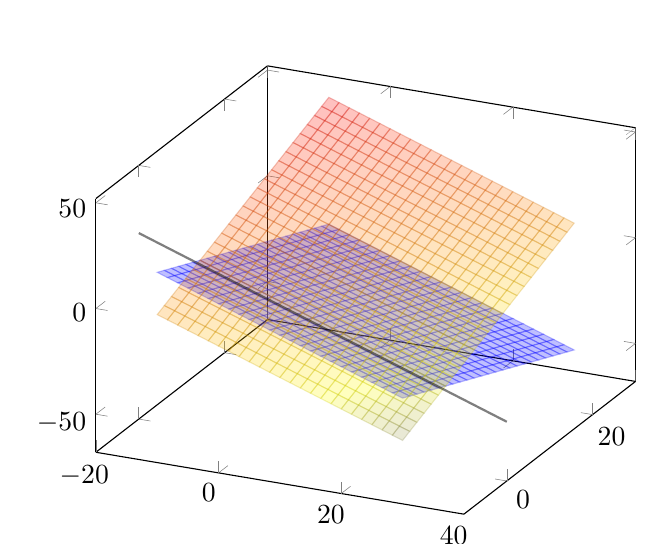
\begin{tikzpicture}
  \begin{axis}[domain=-10:30]
    \addplot3[surf, opacity=0.25, blue, shader=flat] {2-x-y};
    \addplot3[surf, opacity=0.25] {2-x+y};
    \addplot3+[domain=-10:20,samples=80,samples y=0,mark=none,black, opacity=0.5,thick]({2*x},{0.},{-2*x});
  \end{axis}
\end{tikzpicture}

Podkładając vektor (1,0,1) do ograniczeń:

\[1 + 0 + 1 = 2\]
\[1 - 0 + 1 \neq 2\]


\newpage
\section{zadanie 1.4}

Rozwiązanie rozpoczne od wizualizacji problemu na wykresie:

\begin{tikzpicture}
\begin{axis}[view={0}{90},
  domain=0:20 ]
  \addplot3[contour gnuplot={number=14}]
  {6 * x + 6 * y};
  \addplot3[
         color=yellow,
         contour gnuplot={levels={10.0}},
               thick]
                         {x + y};
  \addplot3[
         color=blue,
         contour gnuplot={levels={4.0}},
               thick]
                         {x * -2 + y};
  \end{axis}
\end{tikzpicture}

Z równań oraz rysunku łatwo zauważyć iż prosta ograniczająca x + y = 10 jest linią w której wartość rozwiązania jest stała ( każda prosta o postaci x + y = a jest w tym przypadku jest isolinią).
Z tego wynika że jest ona cała poprawnym rozwiązaniem. Z powodu pozostałych ograniczeń nałożonych na równanie prawidłowym rozwiązaniem będzie zatem odcinek tej prostej.
Zbiór rozwiązań jest zatem następujący:

\[ p = 60 \]
\[ (10 - a, 0 + a); a \in [0, 2] \]

\newpage
\section{zadanie indywidualne}

Zadanie można przedstawić jako funkcję minimalizacji kosztu dostawy makulatury z magazynów do fabryk.

W celu opisania modelu matematycznego wprowadzimy macierz zmiennych:

\[x_{ij}\]

Gdzie i oraz j są kolejno oznaczeniami składnic surowców oraz zakładów przetwórczych.
Zmienna taka określa ilość przeniesionego surowca ze składnicy i do zakładu j.

Z natury zadania wynikają następujące ograniczenia:

\[\forall i\forall j x_{ij} > 0\]

Dodatkowo z treści zadania możemy wyczytać iż odległości pomiędzy składnicami a zakładami są następujące:

{
  \begin{tabular}{|c|c|c|c|c|c|}
    \hline
    & Zakład 1 & Zakład 2 & Zakład 3 & Zakład 4 & Zakład 5 \\ 
    \hline
    Składnica 1 & 130 & 250 & 330 & 170 & 400 \\
    \hline
    Składnica 2 &  290 & 190 & 400 & 260 & 160 \\
    \hline
    Składnica 3 & 150 & 350 & 240 & 190 & 210 \\
    \hline
  \end{tabular}
}

Zauważyć można że odległości można przeskalować przez 1.5 jeśli są mniejsze niż 200 (uzyskamy wtedy koszt transportu jednej tony do danej fabryki) i tak powstaje nowa macierz:

{
  \begin{tabular}{|c|c|c|c|c|c|}
    \hline
    & Zakład 1 & Zakład 2 & Zakład 3 & Zakład 4 & Zakład 5 \\ 
    \hline
    Składnica 1 & 195 & 250 & 330 & 255 & 400 \\
    \hline
    Składnica 2 &  290 & 285 & 400 & 260 & 240 \\
    \hline
    Składnica 3 & 225 & 350 & 240 & 285 & 210 \\
    \hline
  \end{tabular}
}

Kod do znajdowania optymalnego rozwiązania:

\begin{lstlisting}
  param n;
  param p;
  param sums{ i in 1..p};
  param x1{ i in 1..n };
  param x2{ i in 1..n };
  param x3{ i in 1..n };
  param lim{ i in 1..n };
  var v1{ i in 1..n};
  var v2{ i in 1..n};
  var v3{ i in 1..n};

  minimize cost : sum {i in 1..n} v1[i]*x1[i] + sum {i in 1..n} v2[i]*x2[i] + sum {i in 1..n} v3[i]*x3[i] ;

  subject to Dodatniev1 {i in 1..n}: v1[i]>=0;
  subject to Dodatniev2 {i in 1..n}: v2[i]>=0;
  subject to Dodatniev3 {i in 1..n}: v3[i]>=0;
  subject to MaxProd {i in 1..n}: v1[i]+v2[i]+v3[i]<=lim[i];
  subject to Ilosc1: sum {i in 1..n} v1[i] = sums[1];
  subject to Ilosc2: sum {i in 1..n} v2[i] = sums[2];
  subject to Ilosc3: sum {i in 1..n} v3[i] = sums[3];
\end{lstlisting}

Dane podane do programu:

\begin{lstlisting}
param n := 5;
param p := 3;
param sums := 1 500 2 700 3 900;
param x1 := 1 195 2 250 3 330 4 255 5 400;
param x2 := 1 290 2 285 3 400 4 260 5 240;
param x3 := 1 225 2 350 3 240 4 285 5 210;
param lim := 1 400 2 400 3 700 4 300 5 300;
\end{lstlisting}

Znalezione przez program rozwiązanie to 500500;

Wektory określające ilość przewiezionych surowców z magazynów to:

\[v_1 = (400, 100, 0, 0, 0)\]
\[v_2 = (0, 300, 0, 300, 100)\]
\[v_3 = (0, 0, 0, 700, 200)\]

\end{document}
